\documentclass[aspectratio=169]{beamer}
\usepackage{lmodern}
%\usetheme{Madrid}
%\usecolortheme{giantoak}
\newcommand*\oldmacro{}
\let\oldmacro\insertshorttitle
\renewcommand*\insertshorttitle{\oldmacro\hfill\insertframenumber\,/\,\inserttotalframenumber}
\usepackage[framemethod=tikz]{mdframed}

%\usepackage{beamerthemesplit}
\usepackage{textpos}
\usepackage{pgf}
\usepackage{ulem}
%\logo{\pgfputat{\pgfxy(0,-.4)}{\pgfbox[right,base]{\includegraphics[height=1.0cm]{logo.jpg}}}}
%\newcommand{\nologo}{\setbeamertemplate{logo}{}}
\usepackage{booktabs}
\usepackage{graphicx}
\theoremstyle{principle}
\newtheorem*{principle}{Design Principle}


\titlegraphic{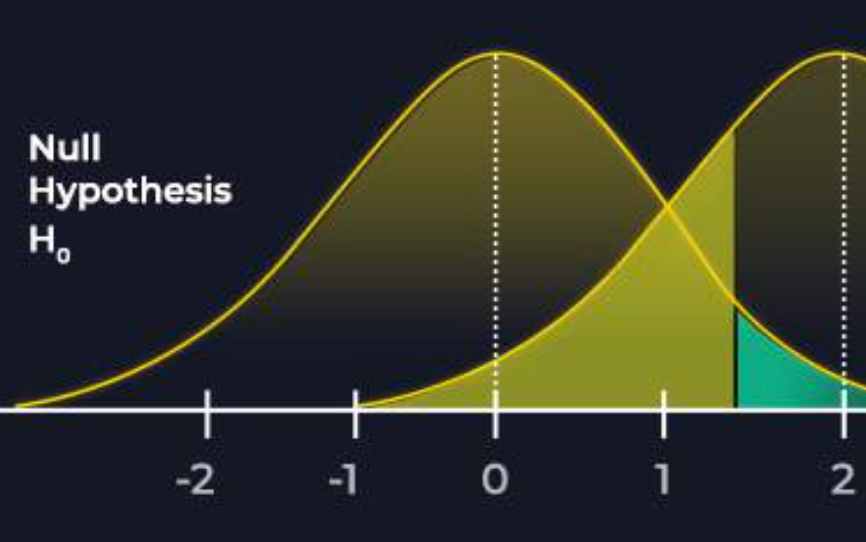
\includegraphics[width=1.0\paperwidth]{distros.png}}

\title{Amendments}
%\author[Jeremy Kedziora]{Wind Data Science Team\\
%\small{Uptake}}
\date{}

\begin{document}

%{
%%\nologo
%\begin{frame}
%    \maketitle
%\end{frame}
%}
%pages 1-7, 8-9, 14-15.


{
%  \usebackgroundtemplate{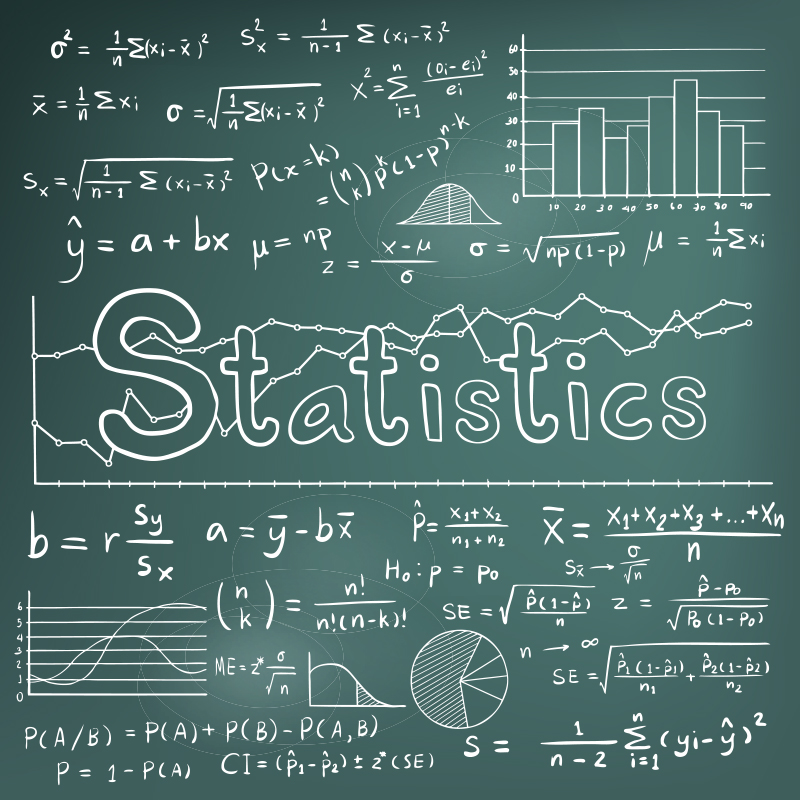
\includegraphics[width=1.0\paperwidth]{statistics-review.jpg}}
  \usebackgroundtemplate{
\includegraphics[scale=0.75]{crazy_curve_2.pdf}}
  \begin{frame}[plain]
  
\begin{mdframed}[tikzsetting={draw=white,fill=white,fill opacity=0.6,draw opacity=0.4,
               line width=0pt},backgroundcolor=none,leftmargin=20,
               rightmargin=20,innertopmargin=4pt]
\begin{center}
\Huge \textbf{Nonlinearity}
\end{center}
\end{mdframed}

  \end{frame}
}

%most reliant on human cognition
%limited only by cognition
%hypothesis generating scheme often functioning as a gateway into more statistical analysis

%%@@@@@@@@@@@@@@@@@@@@@@@@@@@@@@@@@@@@@@@@@@@@@@@@@
%\begin{frame}
%\frametitle{Napoleon's Progress}
%\begin{center}
%
\includegraphics[scale=0.4]{experiment.png}
%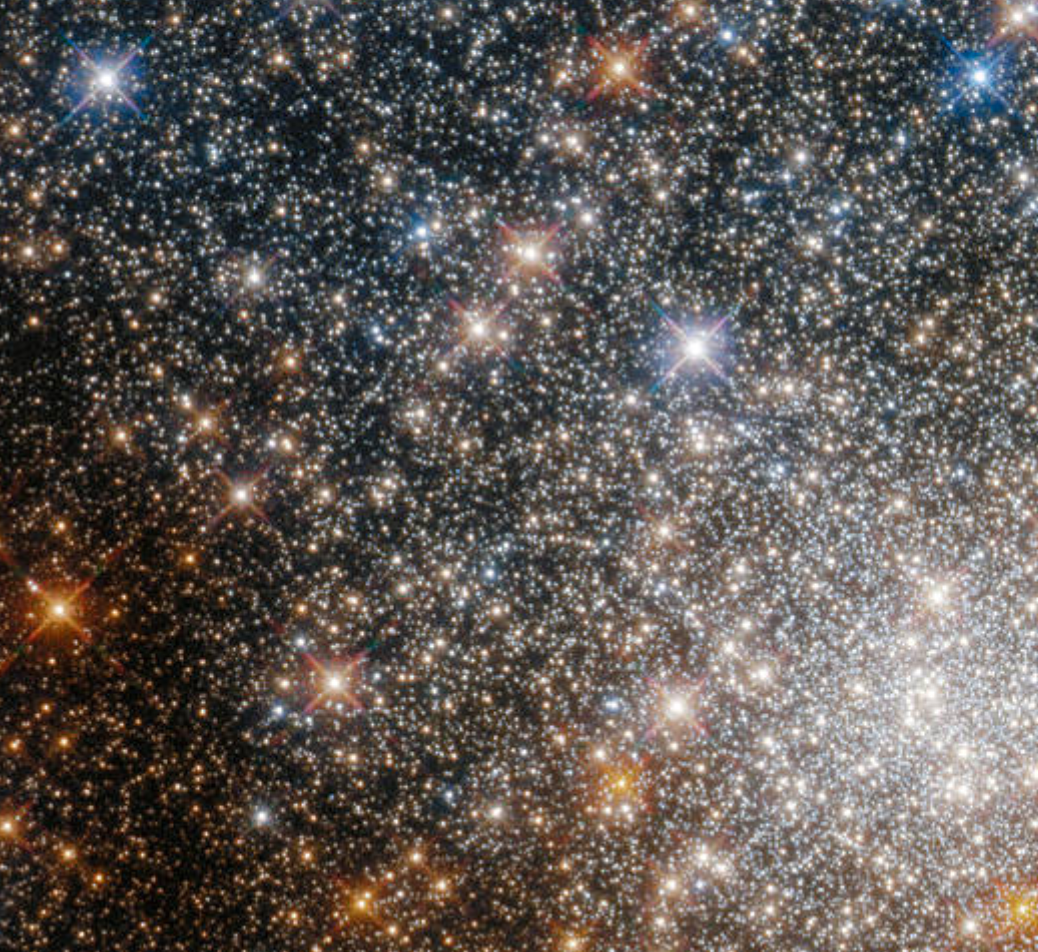
\includegraphics[scale=0.35]{stars.png}
%\end{center}
%
%\end{frame}

%@@@@@@@@@@@@@@@@@@@@@@@@@@@@@@@@@@@@@@@@@@@@@@@@@
\begin{frame}
\frametitle{Today:}

\begin{itemize}
\item Understand some examples of what nonlinearity can look like.
\bigskip
\bigskip
\bigskip

\item Apply two methods for dealing with nonlinearity.

\end{itemize}

\end{frame}

%@@@@@@@@@@@@@@@@@@@@@@@@@@@@@@@@@@@@@@@@@@@@@@@@@
\begin{frame}
\frametitle{What does nonlinearity look like?}

\begin{columns}
\begin{column}{0.4\textwidth}

\begin{itemize}
\item Linear regression allows us to model a linear relationship between $x$ and $y$;
\bigskip
\bigskip
\bigskip

\item[]\color{white} But what if the data looks like this?!

\end{itemize}

\end{column}
\begin{column}{0.6\textwidth}
\begin{center}
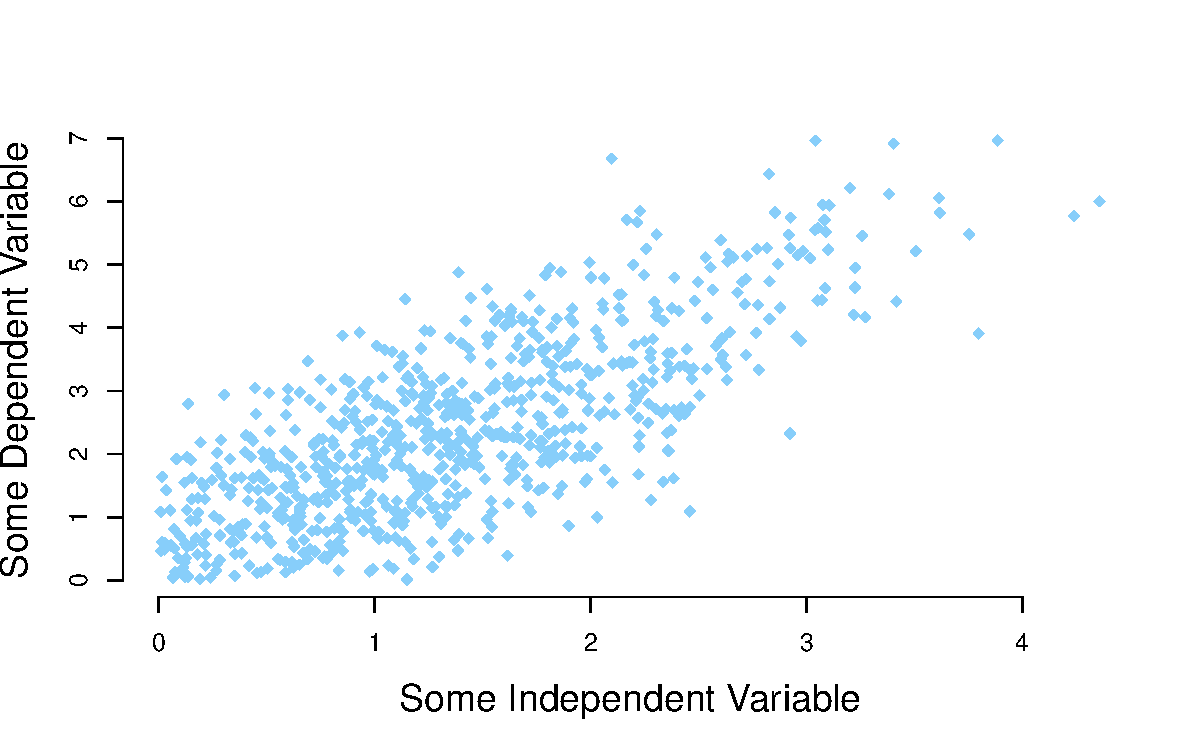
\includegraphics[scale=0.45]{point_cloud.pdf}
\end{center}
\end{column}
\end{columns}

\end{frame}

%@@@@@@@@@@@@@@@@@@@@@@@@@@@@@@@@@@@@@@@@@@@@@@@@@
\begin{frame}
\frametitle{What does nonlinearity look like?}

\begin{columns}
\begin{column}{0.4\textwidth}

\begin{itemize}
\item Linear regression allows us to model a linear relationship between $x$ and $y$;
\bigskip
\bigskip
\bigskip

\item But what if the data looks like this?!

\end{itemize}

\end{column}
\begin{column}{0.6\textwidth}
\begin{center}
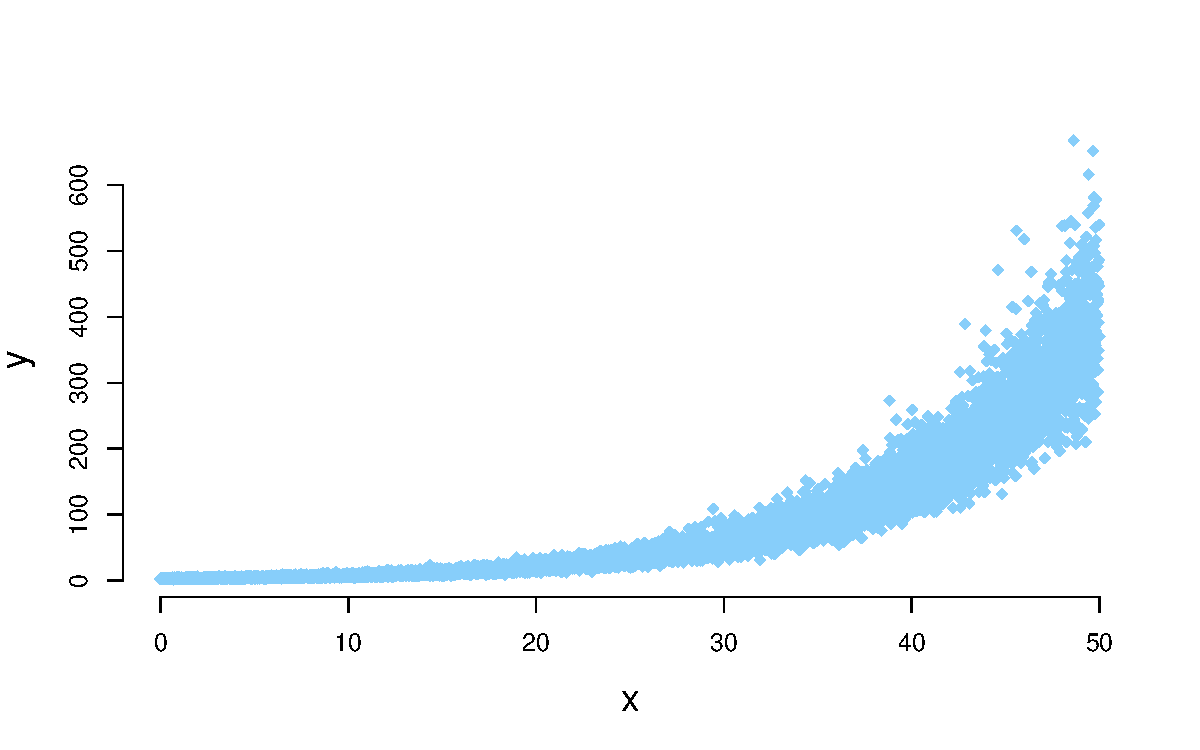
\includegraphics[scale=0.45]{crazy_curve_exp.pdf}
\end{center}
\end{column}
\end{columns}

\end{frame}

%@@@@@@@@@@@@@@@@@@@@@@@@@@@@@@@@@@@@@@@@@@@@@@@@@
\begin{frame}
\frametitle{What does nonlinearity look like?}

\begin{columns}
\begin{column}{0.4\textwidth}

\begin{itemize}
\item Linear regression allows us to model a linear relationship between $x$ and $y$;
\bigskip
\bigskip
\bigskip

\item But what if the data looks like this?!

\end{itemize}

\end{column}
\begin{column}{0.6\textwidth}
\begin{center}
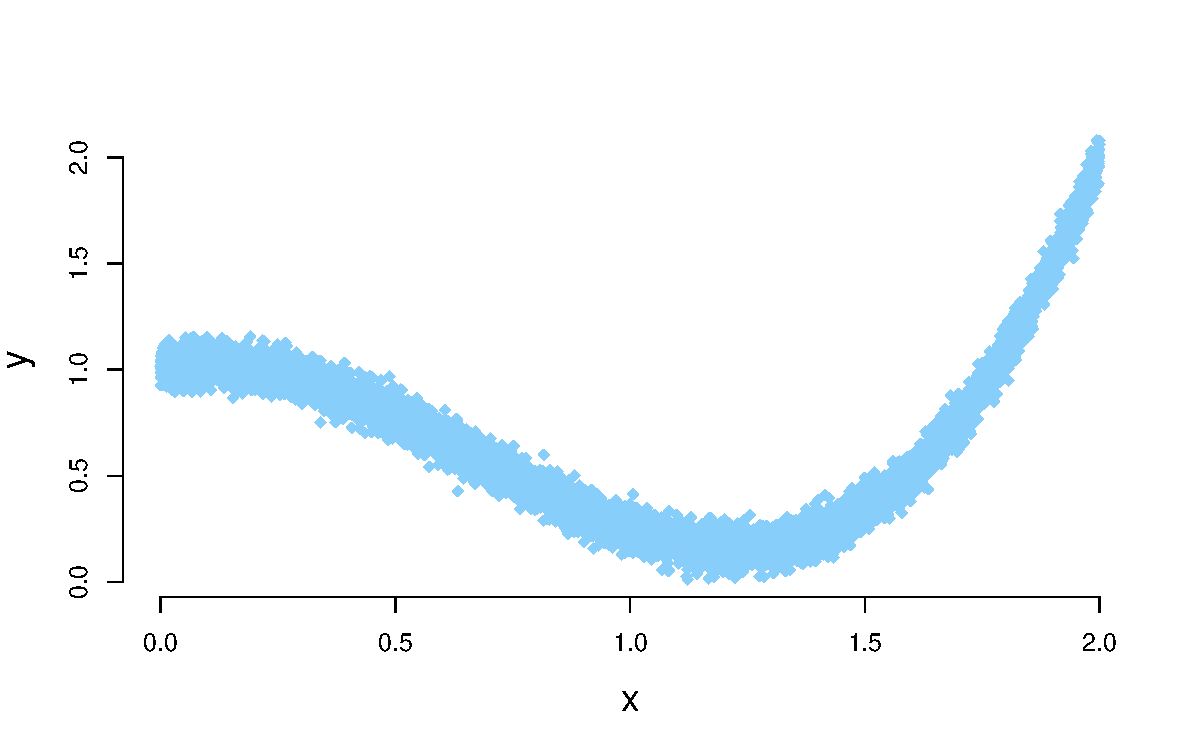
\includegraphics[scale=0.45]{crazy_curve_2_w_axes.pdf}
\end{center}
\end{column}
\end{columns}

\end{frame}

%@@@@@@@@@@@@@@@@@@@@@@@@@@@@@@@@@@@@@@@@@@@@@@@@@
\begin{frame}
\frametitle{Strategy 1 for dealing with nonlinearity}

\begin{itemize}
\item Modify the dependent variable $y$ to turn the nonlinear problem into a linear problem;
\item Very typical to natural log $y$...
\begin{align*}
\mbox{i.e. instead of }y = \beta_0 + \beta_1x + \varepsilon\mbox{ we use: }\ln\{y\} = \beta_0 + \beta_1x + \varepsilon;
\end{align*}
\item Apply linear regression to estimate $\beta_0$ and $\beta_1$;
\item Note -- if you do this you need to be careful with the interpretation of the $\beta$s.  To see this first think about `normal' linear regression:
\begin{align*}
y_1 &= \beta_0 + \beta_1x\\
\color{white}\mbox{for a unit increase in $x$: } y_2 &\color{white}= \beta_0 + \beta_1(x + 1) = \beta_0 + \beta_1x + \beta_1\\
\color{white}\mbox{so change in $y$ is: }y_2 - y_1 &\color{white}= \underbrace{\beta_0 + \beta_1x + \beta_1}_{y_2} - \underbrace{\beta_0 - \beta_1x}_{y_1} = \beta_1.
\end{align*}

\end{itemize}

\end{frame}

%@@@@@@@@@@@@@@@@@@@@@@@@@@@@@@@@@@@@@@@@@@@@@@@@@
\begin{frame}
\frametitle{Strategy 1 for dealing with nonlinearity}

\begin{itemize}
\item Modify the dependent variable $y$ to turn the nonlinear problem into a linear problem;
\item Very typical to natural log $y$...
\begin{align*}
\mbox{i.e. instead of }y = \beta_0 + \beta_1x + \varepsilon\mbox{ we use: }\ln\{y\} = \beta_0 + \beta_1x + \varepsilon;
\end{align*}
\item Apply linear regression to estimate $\beta_0$ and $\beta_1$;
\item Note -- if you do this you need to be careful with the interpretation of the $\beta$s.  To see this first think about `normal' linear regression:
\begin{align*}
y_1 &= \beta_0 + \beta_1x\\
\mbox{for a unit increase in $x$: } y_2 &= \beta_0 + \beta_1(x + 1)\color{white} = \beta_0 + \beta_1x + \beta_1\\
\color{white}\mbox{so change in $y$ is: }y_2 - y_1 &\color{white}= \underbrace{\beta_0 + \beta_1x + \beta_1}_{y_2} - \underbrace{\beta_0 - \beta_1x}_{y_1} = \beta_1.
\end{align*}

\end{itemize}

\end{frame}

%@@@@@@@@@@@@@@@@@@@@@@@@@@@@@@@@@@@@@@@@@@@@@@@@@
\begin{frame}
\frametitle{Strategy 1 for dealing with nonlinearity}

\begin{itemize}
\item Modify the dependent variable $y$ to turn the nonlinear problem into a linear problem;
\item Very typical to natural log $y$...
\begin{align*}
\mbox{i.e. instead of }y = \beta_0 + \beta_1x + \varepsilon\mbox{ we use: }\ln\{y\} = \beta_0 + \beta_1x + \varepsilon;
\end{align*}
\item Apply linear regression to estimate $\beta_0$ and $\beta_1$;
\item Note -- if you do this you need to be careful with the interpretation of the $\beta$s.  To see this first think about `normal' linear regression:
\begin{align*}
y_1 &= \beta_0 + \beta_1x\\
\mbox{for a unit increase in $x$: } y_2 &= \beta_0 + \beta_1(x + 1) = \beta_0 + \beta_1x + \beta_1\\
\color{white}\mbox{so change in $y$ is: }y_2 - y_1 &\color{white}= \underbrace{\beta_0 + \beta_1x + \beta_1}_{y_2} - \underbrace{\beta_0 - \beta_1x}_{y_1} = \beta_1.
\end{align*}

\end{itemize}

\end{frame}

%@@@@@@@@@@@@@@@@@@@@@@@@@@@@@@@@@@@@@@@@@@@@@@@@@
\begin{frame}
\frametitle{Strategy 1 for dealing with nonlinearity}

\begin{itemize}
\item Modify the dependent variable $y$ to turn the nonlinear problem into a linear problem;
\item Very typical to natural log $y$...
\begin{align*}
\mbox{i.e. instead of }y = \beta_0 + \beta_1x + \varepsilon\mbox{ we use: }\ln\{y\} = \beta_0 + \beta_1x + \varepsilon;
\end{align*}
\item Apply linear regression to estimate $\beta_0$ and $\beta_1$;
\item Note -- if you do this you need to be careful with the interpretation of the $\beta$s.  To see this first think about `normal' linear regression:
\begin{align*}
y_1 &= \beta_0 + \beta_1x\\
\mbox{for a unit increase in $x$: } y_2 &= \beta_0 + \beta_1(x + 1) = \beta_0 + \beta_1x + \beta_1\\
\mbox{so change in $y$ is: }y_2 - y_1 &\color{white}= \underbrace{\beta_0 + \beta_1x + \beta_1}_{y_2} - \underbrace{\beta_0 - \beta_1x}_{y_1} = \beta_1.
\end{align*}

\end{itemize}

\end{frame}

%@@@@@@@@@@@@@@@@@@@@@@@@@@@@@@@@@@@@@@@@@@@@@@@@@
\begin{frame}
\frametitle{Strategy 1 for dealing with nonlinearity}

\begin{itemize}
\item Modify the dependent variable $y$ to turn the nonlinear problem into a linear problem;
\item Very typical to natural log $y$...
\begin{align*}
\mbox{i.e. instead of }y = \beta_0 + \beta_1x + \varepsilon\mbox{ we use: }\ln\{y\} = \beta_0 + \beta_1x + \varepsilon;
\end{align*}
\item Apply linear regression to estimate $\beta_0$ and $\beta_1$;
\item Note -- if you do this you need to be careful with the interpretation of the $\beta$s.  To see this first think about `normal' linear regression:
\begin{align*}
y_1 &= \beta_0 + \beta_1x\\
\mbox{for a unit increase in $x$: } y_2 &= \beta_0 + \beta_1(x + 1) = \beta_0 + \beta_1x + \beta_1\\
\mbox{so change in $y$ is: }y_2 - y_1 &= \underbrace{\beta_0 + \beta_1x + \beta_1}_{y_2} - \underbrace{\beta_0 - \beta_1x}_{y_1} = \beta_1.
\end{align*}

\end{itemize}

\end{frame}

%@@@@@@@@@@@@@@@@@@@@@@@@@@@@@@@@@@@@@@@@@@@@@@@@@
\begin{frame}
\frametitle{Strategy 1 for dealing with nonlinearity}

\begin{itemize}
\item Modify the dependent variable $y$ to turn the nonlinear problem into a linear problem;
\item Very typical to natural log $y$...
\begin{align*}
\mbox{i.e. instead of }y = \beta_0 + \beta_1x + \varepsilon\mbox{ we use: }\ln\{y\} = \beta_0 + \beta_1x + \varepsilon;
\end{align*}
\item Apply linear regression to estimate $\beta_0$ and $\beta_1$;
\item Note -- if you do this you need to be careful with the interpretation of the $\beta$s.  Now think about `logged' linear regression:
\begin{align*}
\ln\{y_1\} &= \beta_0 + \beta_1x\\
\color{white}\mbox{for a unit increase in $x$: } \ln\{y_2\} &\color{white}= \beta_0 + \beta_1(x + 1) = \beta_0 + \beta_1x + \beta_1\\
\color{white}\mbox{so change in $y$ is: }y_2 - y_1 &\color{white}= \underbrace{\exp\{\beta_1\}\exp\{\beta_0 + \beta_1x)\}}_{y_2} - \underbrace{\exp\{\beta_0 + \beta_1x\}}_{y_1}
\end{align*}

\end{itemize}

\end{frame}

%@@@@@@@@@@@@@@@@@@@@@@@@@@@@@@@@@@@@@@@@@@@@@@@@@
\begin{frame}
\frametitle{Strategy 1 for dealing with nonlinearity}

\begin{itemize}
\item Modify the dependent variable $y$ to turn the nonlinear problem into a linear problem;
\item Very typical to natural log $y$...
\begin{align*}
\mbox{i.e. instead of }y = \beta_0 + \beta_1x + \varepsilon\mbox{ we use: }\ln\{y\} = \beta_0 + \beta_1x + \varepsilon;
\end{align*}
\item Apply linear regression to estimate $\beta_0$ and $\beta_1$;
\item Note -- if you do this you need to be careful with the interpretation of the $\beta$s.  Now think about `logged' linear regression:
\begin{align*}
\ln\{y_1\} &= \beta_0 + \beta_1x\\
\mbox{for a unit increase in $x$: } \ln\{y_2\} &= \beta_0 + \beta_1(x + 1)\color{white} = \beta_0 + \beta_1x + \beta_1\\
\color{white}\mbox{so change in $y$ is: }y_2 - y_1 &\color{white}= \underbrace{\exp\{\beta_1\}\exp\{\beta_0 + \beta_1x)\}}_{y_2} - \underbrace{\exp\{\beta_0 + \beta_1x\}}_{y_1}
\end{align*}

\end{itemize}

\end{frame}

%@@@@@@@@@@@@@@@@@@@@@@@@@@@@@@@@@@@@@@@@@@@@@@@@@
\begin{frame}
\frametitle{Strategy 1 for dealing with nonlinearity}

\begin{itemize}
\item Modify the dependent variable $y$ to turn the nonlinear problem into a linear problem;
\item Very typical to natural log $y$...
\begin{align*}
\mbox{i.e. instead of }y = \beta_0 + \beta_1x + \varepsilon\mbox{ we use: }\ln\{y\} = \beta_0 + \beta_1x + \varepsilon;
\end{align*}
\item Apply linear regression to estimate $\beta_0$ and $\beta_1$;
\item Note -- if you do this you need to be careful with the interpretation of the $\beta$s.  Now think about `logged' linear regression:
\begin{align*}
\ln\{y_1\} &= \beta_0 + \beta_1x\\
\mbox{for a unit increase in $x$: } \ln\{y_2\} &= \beta_0 + \beta_1(x + 1) = \beta_0 + \beta_1x + \beta_1\\
\color{white}\mbox{so change in $y$ is: }y_2 - y_1 &\color{white}= \underbrace{\exp\{\beta_1\}\exp\{\beta_0 + \beta_1x)\}}_{y_2} - \underbrace{\exp\{\beta_0 + \beta_1x\}}_{y_1}
\end{align*}

\end{itemize}

\end{frame}

%@@@@@@@@@@@@@@@@@@@@@@@@@@@@@@@@@@@@@@@@@@@@@@@@@
\begin{frame}
\frametitle{Strategy 1 for dealing with nonlinearity}

\begin{itemize}
\item Modify the dependent variable $y$ to turn the nonlinear problem into a linear problem;
\item Very typical to natural log $y$...
\begin{align*}
\mbox{i.e. instead of }y = \beta_0 + \beta_1x + \varepsilon\mbox{ we use: }\ln\{y\} = \beta_0 + \beta_1x + \varepsilon;
\end{align*}
\item Apply linear regression to estimate $\beta_0$ and $\beta_1$;
\item Note -- if you do this you need to be careful with the interpretation of the $\beta$s.  Now think about `logged' linear regression:
\begin{align*}
\exp\{\ln\{y_1\}\} &= \exp\{\beta_0 + \beta_1x\}\\
\mbox{for a unit increase in $x$: } \exp\{\ln\{y_2\}\} &= \exp\{\beta_0 + \beta_1(x + 1)\} = \exp\{\beta_0 + \beta_1x + \beta_1\}\\
\color{white}\mbox{so change in $y$ is: }y_2 - y_1 &\color{white}= \underbrace{\exp\{\beta_1\}\exp\{\beta_0 + \beta_1x)\}}_{y_2} - \underbrace{\exp\{\beta_0 + \beta_1x\}}_{y_1}
\end{align*}

\end{itemize}

\end{frame}

%@@@@@@@@@@@@@@@@@@@@@@@@@@@@@@@@@@@@@@@@@@@@@@@@@
\begin{frame}
\frametitle{Strategy 1 for dealing with nonlinearity}

\begin{itemize}
\item Modify the dependent variable $y$ to turn the nonlinear problem into a linear problem;
\item Very typical to natural log $y$...
\begin{align*}
\mbox{i.e. instead of }y = \beta_0 + \beta_1x + \varepsilon\mbox{ we use: }\ln\{y\} = \beta_0 + \beta_1x + \varepsilon;
\end{align*}
\item Apply linear regression to estimate $\beta_0$ and $\beta_1$;
\item Note -- if you do this you need to be careful with the interpretation of the $\beta$s.  Now think about `logged' linear regression:
\begin{align*}
y_1 &= \exp\{\beta_0 + \beta_1x\}\\
\mbox{for a unit increase in $x$: } y_2 &= \exp\{\beta_0 + \beta_1(x + 1)\} = \exp\{\beta_0 + \beta_1x + \beta_1\}\\
\color{white}\mbox{so change in $y$ is: }y_2 - y_1 &\color{white}= \underbrace{\exp\{\beta_1\}\exp\{\beta_0 + \beta_1x)\}}_{y_2} - \underbrace{\exp\{\beta_0 + \beta_1x\}}_{y_1}
\end{align*}

\end{itemize}

\end{frame}

%@@@@@@@@@@@@@@@@@@@@@@@@@@@@@@@@@@@@@@@@@@@@@@@@@
\begin{frame}
\frametitle{Strategy 1 for dealing with nonlinearity}

\begin{itemize}
\item Modify the dependent variable $y$ to turn the nonlinear problem into a linear problem;
\item Very typical to natural log $y$...
\begin{align*}
\mbox{i.e. instead of }y = \beta_0 + \beta_1x + \varepsilon\mbox{ we use: }\ln\{y\} = \beta_0 + \beta_1x + \varepsilon;
\end{align*}
\item Apply linear regression to estimate $\beta_0$ and $\beta_1$;
\item Note -- if you do this you need to be careful with the interpretation of the $\beta$s.  Now think about `logged' linear regression:
\begin{align*}
y_1 &= \exp\{\beta_0 + \beta_1x\}\\
\mbox{for a unit increase in $x$: } y_2 &= \exp\{\beta_0 + \beta_1(x + 1)\} = \exp\{\beta_1\}\exp\{\beta_0 + \beta_1x\}\\
\color{white}\mbox{so change in $y$ is: }y_2 - y_1 &\color{white}= \underbrace{\exp\{\beta_1\}\exp\{\beta_0 + \beta_1x)\}}_{y_2} - \underbrace{\exp\{\beta_0 + \beta_1x\}}_{y_1}
\end{align*}

\end{itemize}

\end{frame}

%@@@@@@@@@@@@@@@@@@@@@@@@@@@@@@@@@@@@@@@@@@@@@@@@@
\begin{frame}
\frametitle{Strategy 1 for dealing with nonlinearity}

\begin{itemize}
\item Modify the dependent variable $y$ to turn the nonlinear problem into a linear problem;
\item Very typical to natural log $y$...
\begin{align*}
\mbox{i.e. instead of }y = \beta_0 + \beta_1x + \varepsilon\mbox{ we use: }\ln\{y\} = \beta_0 + \beta_1x + \varepsilon;
\end{align*}
\item Apply linear regression to estimate $\beta_0$ and $\beta_1$;
\item Note -- if you do this you need to be careful with the interpretation of the $\beta$s.  Now think about `logged' linear regression:
\begin{align*}
y_1 &= \exp\{\beta_0 + \beta_1x\}\\
\mbox{for a unit increase in $x$: } y_2 &= \exp\{\beta_0 + \beta_1(x)\} = \exp\{\beta_1\}\exp\{\beta_0 + \beta_1x)\}\\
\mbox{so change in $y$ is: }y_2 - y_1 &\color{white}= \underbrace{\exp\{\beta_1\}\exp\{\beta_0 + \beta_1x)\}}_{y_2} - \underbrace{\exp\{\beta_0 + \beta_1x\}}_{y_1}
\end{align*}

\end{itemize}

\end{frame}

%@@@@@@@@@@@@@@@@@@@@@@@@@@@@@@@@@@@@@@@@@@@@@@@@@
\begin{frame}
\frametitle{Strategy 1 for dealing with nonlinearity}

\begin{itemize}
\item Modify the dependent variable $y$ to turn the nonlinear problem into a linear problem;
\item Very typical to natural log $y$...
\begin{align*}
\mbox{i.e. instead of }y = \beta_0 + \beta_1x + \varepsilon\mbox{ we use: }\ln\{y\} = \beta_0 + \beta_1x + \varepsilon;
\end{align*}
\item Apply linear regression to estimate $\beta_0$ and $\beta_1$;
\item Note -- if you do this you need to be careful with the interpretation of the $\beta$s.  Now think about `logged' linear regression:
\begin{align*}
y_1 &= \exp\{\beta_0 + \beta_1x\}\\
\mbox{for a unit increase in $x$: } y_2 &= \exp\{\beta_0 + \beta_1(x)\} = \exp\{\beta_1\}\exp\{\beta_0 + \beta_1x)\}\\
\mbox{so change in $y$ is: }y_2 - y_1 &= \underbrace{\exp\{\beta_1\}\exp\{\beta_0 + \beta_1x)\}}_{y_2} - \underbrace{\exp\{\beta_0 + \beta_1x\}}_{y_1}
\end{align*}

\end{itemize}

\end{frame}

%@@@@@@@@@@@@@@@@@@@@@@@@@@@@@@@@@@@@@@@@@@@@@@@@@
\begin{frame}
\frametitle{Strategy 1 for dealing with nonlinearity}

\begin{itemize}
\item Modify the dependent variable $y$ to turn the nonlinear problem into a linear problem;
\item Very typical to natural log $y$...
\begin{align*}
\mbox{i.e. instead of }y = \beta_0 + \beta_1x + \varepsilon\mbox{ we use: }\ln\{y\} = \beta_0 + \beta_1x + \varepsilon;
\end{align*}
\item Apply linear regression to estimate $\beta_0$ and $\beta_1$;
\item Note -- if you do this you need to be careful with the interpretation of the $\beta$s.  Now think about `logged' linear regression:
\begin{align*}
y_1 &= \exp\{\beta_0 + \beta_1x\}\\
\mbox{for a unit increase in $x$: } y_2 &= \exp\{\beta_0 + \beta_1(x)\} = \exp\{\beta_1\}\exp\{\beta_0 + \beta_1x)\}\\
\mbox{so change in $y$ is: }y_2 - y_1 &= (\exp\{\beta_1\}  - 1)\exp\{\beta_0 + \beta_1x)\}.
\end{align*}

\end{itemize}

\end{frame}

%@@@@@@@@@@@@@@@@@@@@@@@@@@@@@@@@@@@@@@@@@@@@@@@@@
\begin{frame}
\frametitle{Strategy 1 for dealing with nonlinearity}

\begin{center}
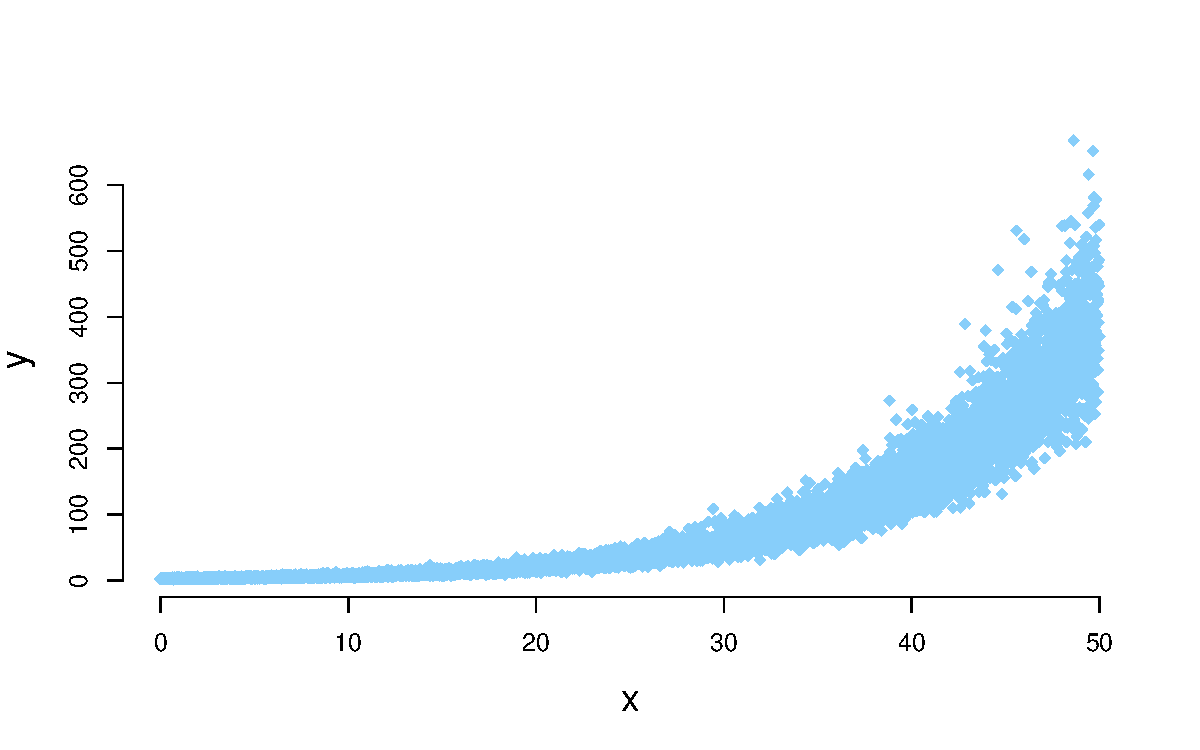
\includegraphics[scale=0.6]{crazy_curve_exp.pdf}
\end{center}

\end{frame}

%@@@@@@@@@@@@@@@@@@@@@@@@@@@@@@@@@@@@@@@@@@@@@@@@@
\begin{frame}
\frametitle{Strategy 1 for dealing with nonlinearity}

\begin{center}
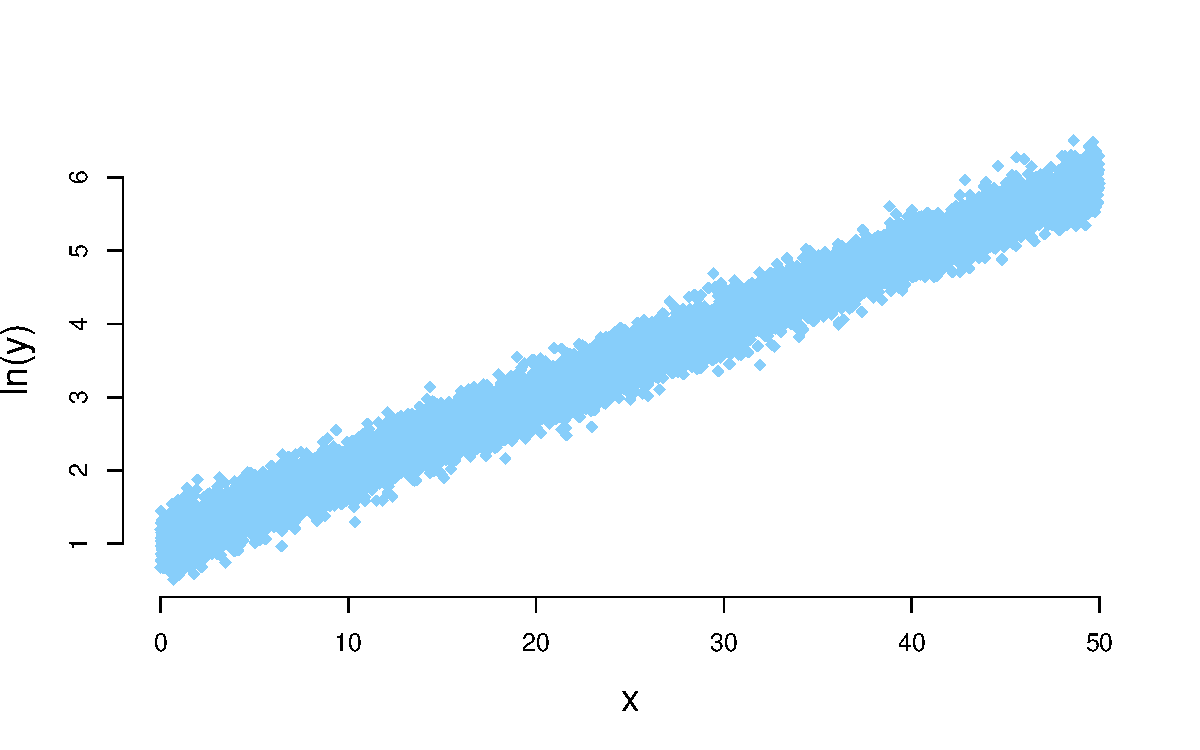
\includegraphics[scale=0.6]{crazy_curve_exp_logged.pdf}
\end{center}

\end{frame}

%@@@@@@@@@@@@@@@@@@@@@@@@@@@@@@@@@@@@@@@@@@@@@@@@@
\begin{frame}
\frametitle{Strategy 2 for dealing with nonlinearity}

\begin{itemize}
\item Modify the independent variable $x$ to model the nonlinearity;
\bigskip

\item Very typical to use a polynomial of $x$, for example $x^2$ or $x^3$:
\begin{align*}
y = \beta_0 + \beta_1x + \beta_2x^2 + \beta_3x^3 + \varepsilon
\end{align*}

\item Apply linear regression to estimate $\beta$s;
\bigskip

\item Note -- if you do this do not extrapolate beyond the boundary of the sample.
\end{itemize}

\end{frame}

%@@@@@@@@@@@@@@@@@@@@@@@@@@@@@@@@@@@@@@@@@@@@@@@@@
\begin{frame}
\frametitle{Strategy 2 for dealing with nonlinearity}

\begin{columns}
\begin{column}{0.3\textwidth}



\end{column}
\begin{column}{0.7\textwidth}

\begin{center}
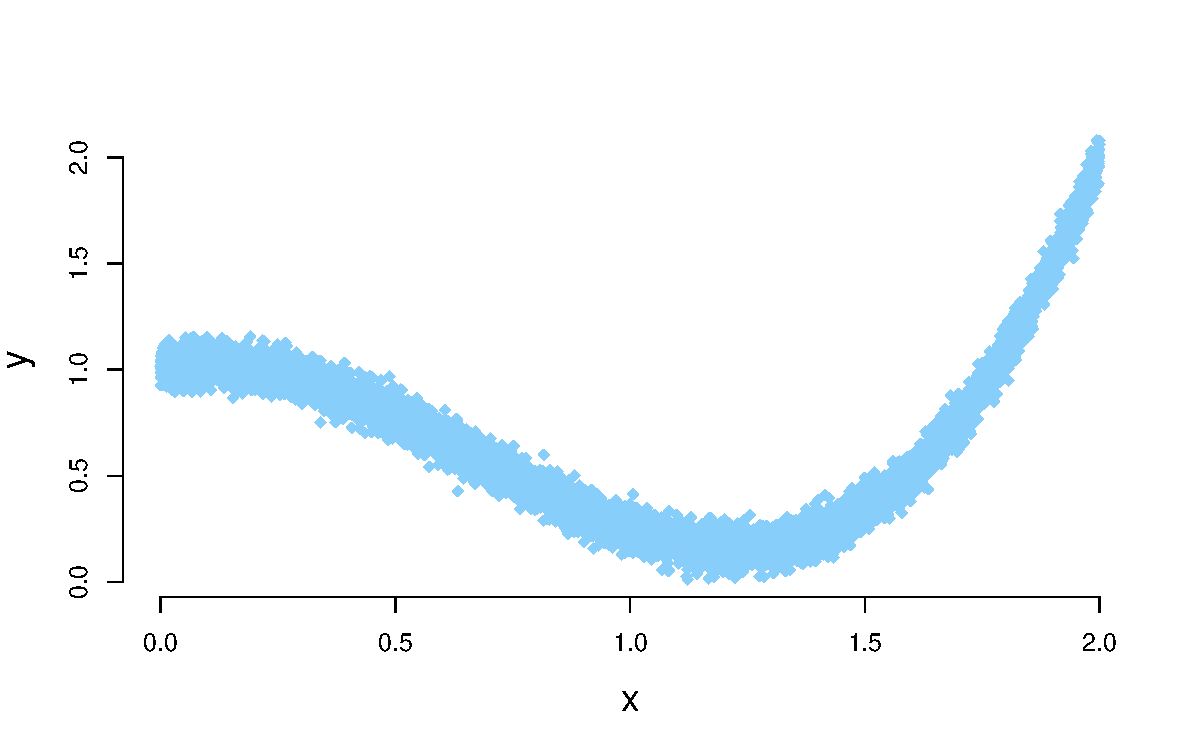
\includegraphics[scale=0.5]{crazy_curve_2_w_axes.pdf}
\end{center}

\end{column}
\end{columns}

\end{frame}

%@@@@@@@@@@@@@@@@@@@@@@@@@@@@@@@@@@@@@@@@@@@@@@@@@
\begin{frame}
\frametitle{What about a simple \textbf{linear} model?}

\begin{columns}
\begin{column}{0.3\textwidth}

\begin{center}
\begin{tabular}{ lrl } 
\hline
\hline
 & Coefficient & $p$-value\\ 
Incpt & 0.6750 & 0.0\\ 
$x$ & -0.0096 & 0.185 \\ 
\hline
\hline
\end{tabular}
\end{center}

\end{column}
\begin{column}{0.7\textwidth}

\begin{center}
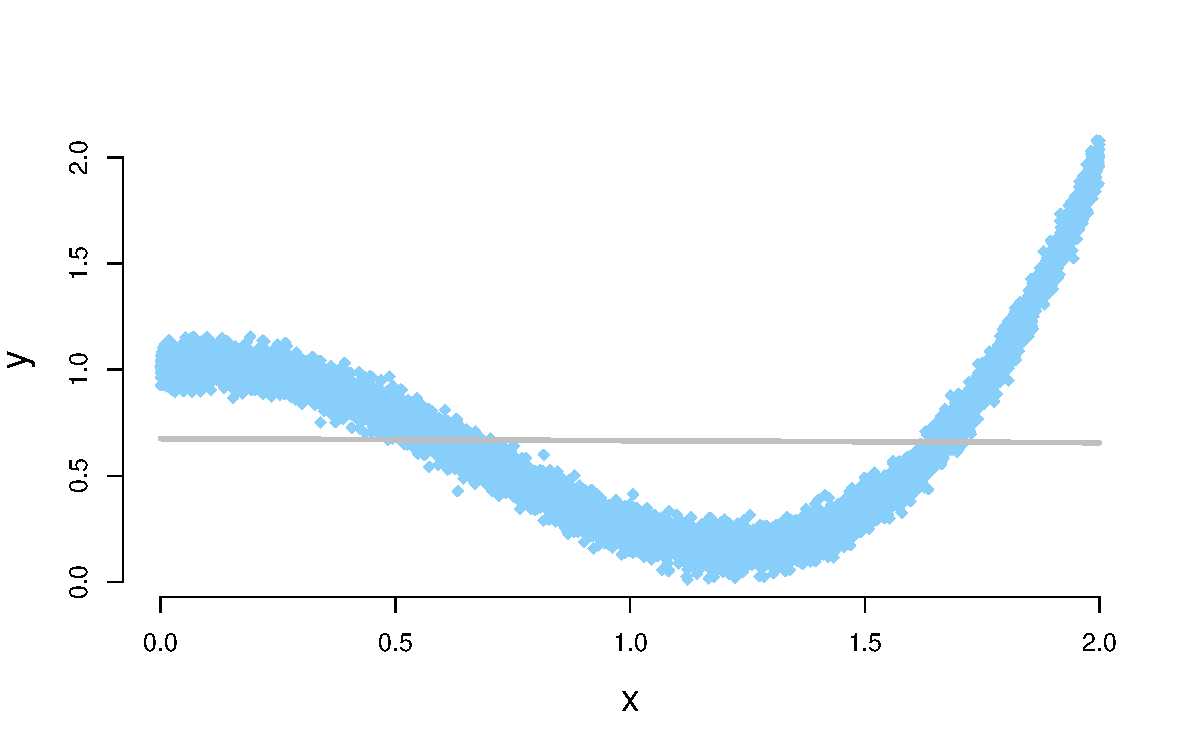
\includegraphics[scale=0.5]{crazy_curve_x.pdf}
\end{center}

\end{column}
\end{columns}

\end{frame}

%@@@@@@@@@@@@@@@@@@@@@@@@@@@@@@@@@@@@@@@@@@@@@@@@@
\begin{frame}
\frametitle{What about a \textbf{quadratic} model?}

\begin{columns}
\begin{column}{0.3\textwidth}

\begin{center}
\begin{tabular}{ lrl } 
\hline
\hline
 & Coefficient & $p$-value\\ 
Incpt & 1.4952 & 0.0\\ 
$x$ & -2.4825 &0.0\\ 
$x^2$ & 1.2409 &0.0\\ 
\hline
\hline
\end{tabular}
\end{center}

\end{column}
\begin{column}{0.7\textwidth}

\begin{center}
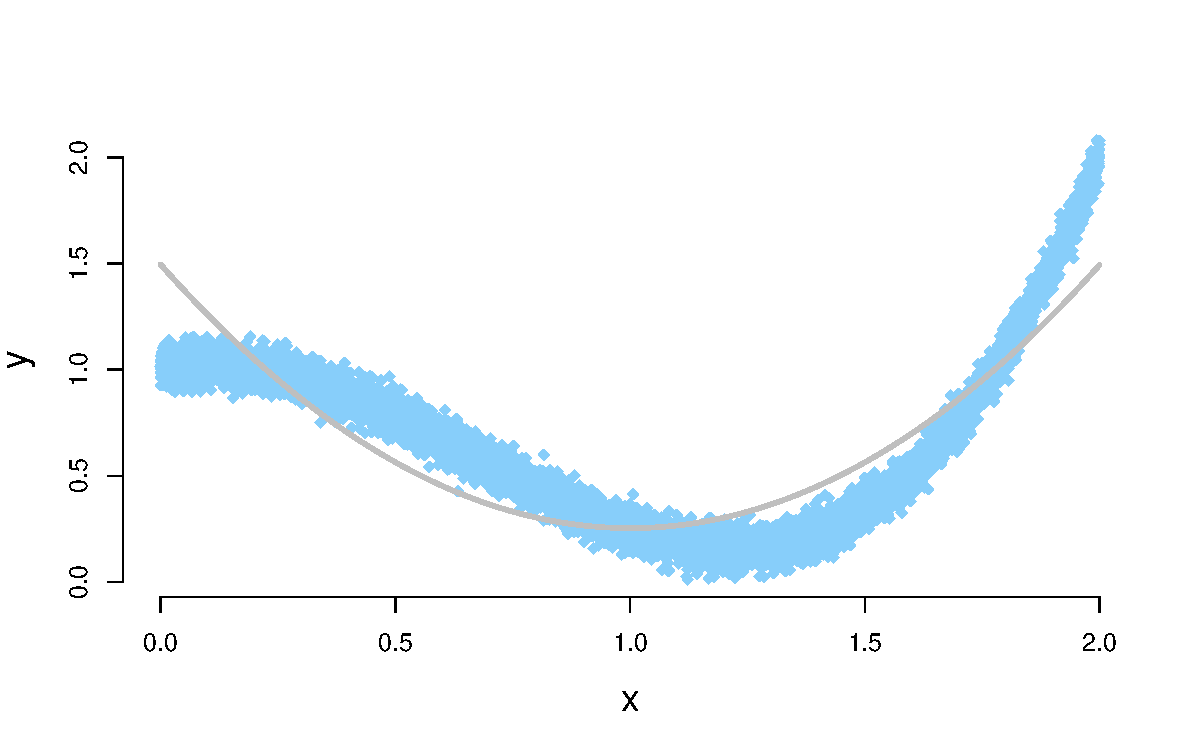
\includegraphics[scale=0.5]{crazy_curve_x2.pdf}
\end{center}

\end{column}
\end{columns}

\end{frame}

%@@@@@@@@@@@@@@@@@@@@@@@@@@@@@@@@@@@@@@@@@@@@@@@@@
\begin{frame}
\frametitle{What about a \textbf{cubic polynomial} model?}

\begin{columns}
\begin{column}{0.3\textwidth}

\begin{center}
\begin{tabular}{ lrl } 
\hline
\hline
 & Coefficient & $p$-value\\ 
Incpt & 1.0012 &0.0\\ 
$x$ & 0.4934 &0.0\\ 
$x^2$ & -2.4914 &0.0\\ 
$x^3$ & 1.2469 &0.0\\ 
\hline
\hline
\end{tabular}
\end{center}

\end{column}
\begin{column}{0.7\textwidth}

\begin{center}
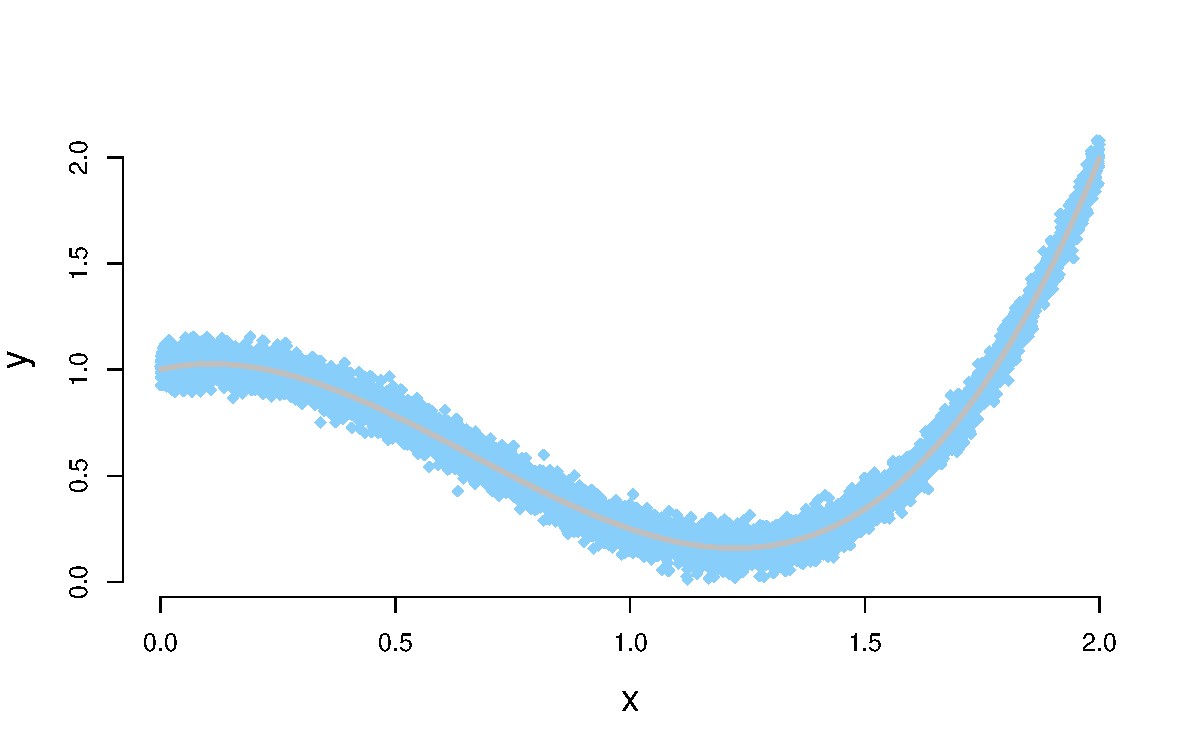
\includegraphics[scale=0.5]{crazy_curve_x3.pdf}
\end{center}

\end{column}
\end{columns}

\end{frame}

%@@@@@@@@@@@@@@@@@@@@@@@@@@@@@@@@@@@@@@@@@@@@@@@@@
\begin{frame}
\frametitle{Here is the true model: $y=1.0 + 0.5x - 2.5x^2 + 1.25x^3 + \varepsilon$.}

\begin{columns}
\begin{column}{0.3\textwidth}

\begin{center}
\begin{tabular}{ lrl } 
\hline
\hline
 & Coefficient & $p$-value\\ 
Incpt & 1.0 &0.0\\ 
$x$ & 0.5 &0.0\\ 
$x^2$ & -2.5 &0.0\\ 
$x^3$ & 1.25 &0.0\\ 
\hline
\hline
\end{tabular}
\end{center}

\end{column}
\begin{column}{0.7\textwidth}

\begin{center}
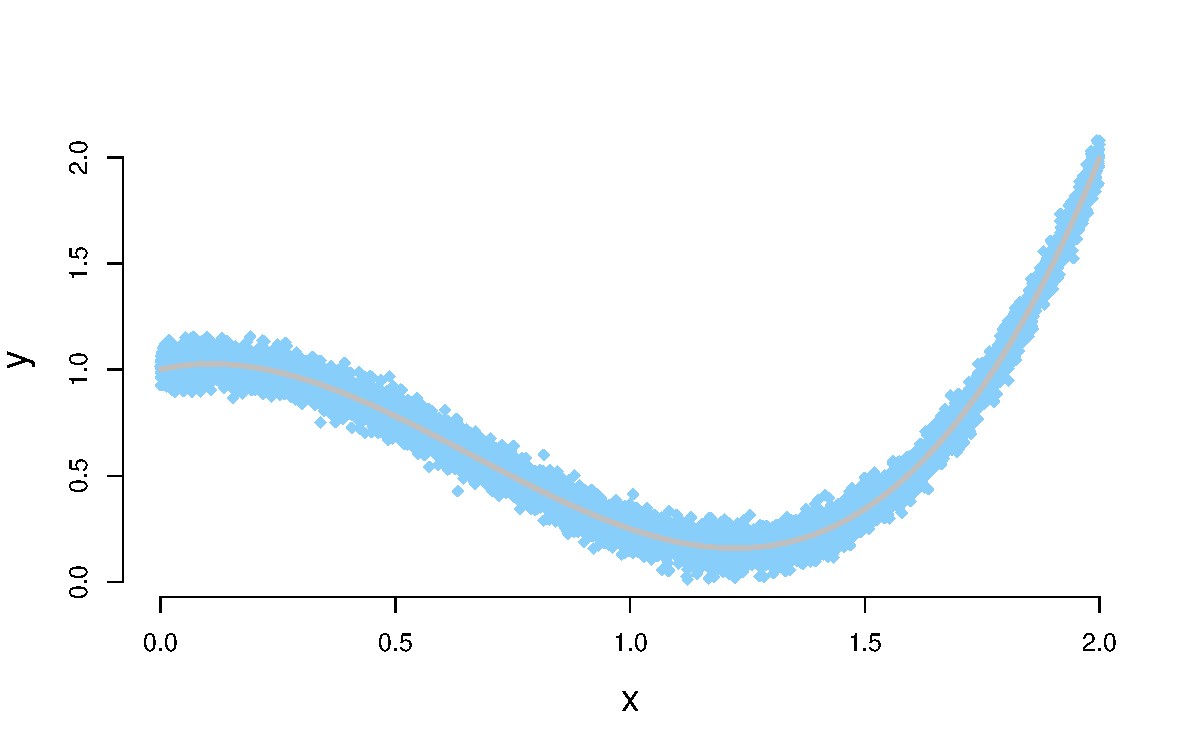
\includegraphics[scale=0.5]{crazy_curve_x3.pdf}
\end{center}

\end{column}
\end{columns}

\end{frame}

%\item Remember the \textbf{binomial distribution} that models the probability of $k$ successes in $n$ trials given that each trial has probability of success $\pi$?
%\bigskip
%\bigskip
%
%\item Let's use this to compute the null distribution (the distribution over the number of Johnson voters in a sample of 15 given that $H_0$ is true so that $\pi = 0.5$).
%\bigskip

%%@@@@@@@@@@@@@@@@@@@@@@@@@@@@@@@@@@@@@@@@@@@@@@@@@
%\begin{frame}
%\frametitle{An IRL example: polling in 1936...}
%
%\begin{columns}
%\begin{column}{0.5\textwidth}
%
%\begin{itemize}
%\item Blar;
%
%\item Blar;
%
%\item Blar;
%
%\end{itemize}
%
%\end{column}
%\begin{column}{0.5\textwidth}
%\begin{center}
%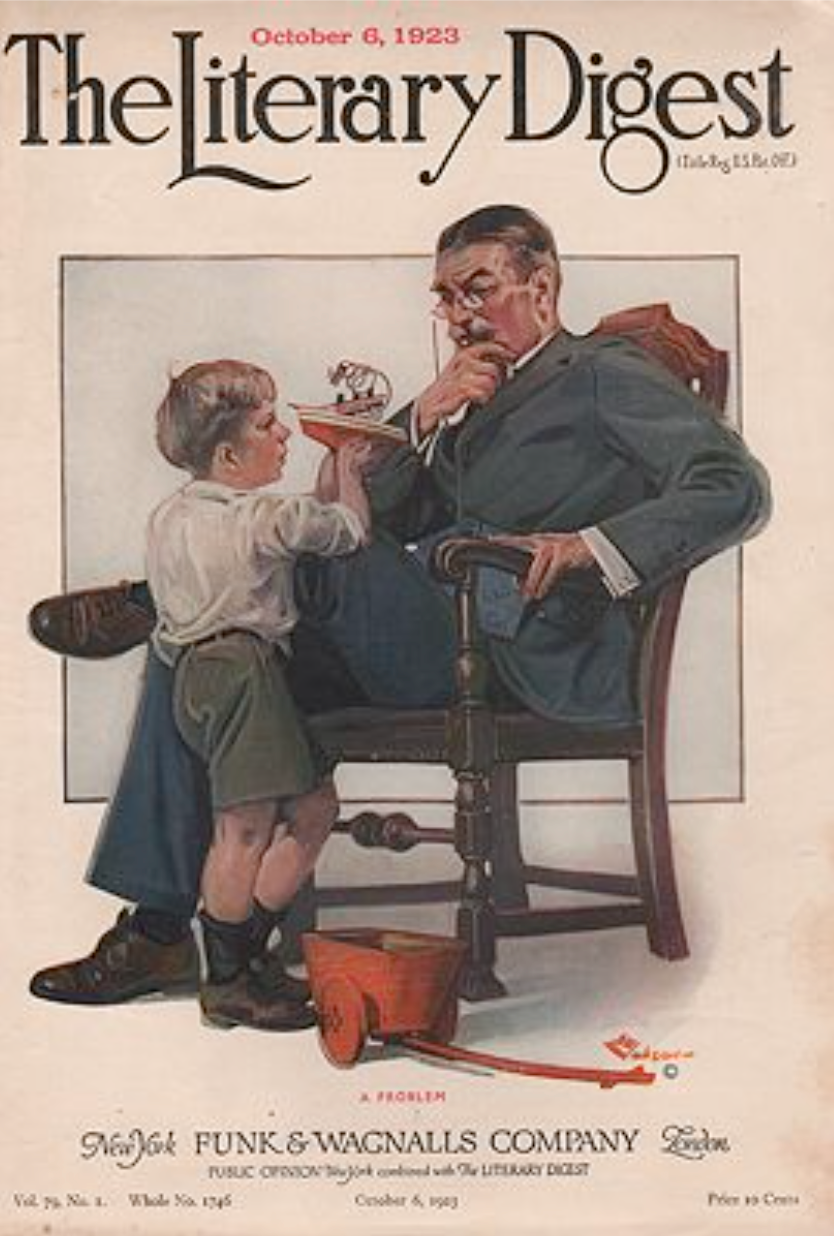
\includegraphics[scale=0.3]{LD.png}
%\end{center}
%\end{column}
%\end{columns}
%
%\end{frame}

%@@@@@@@@@@@@@@@@@@@@@@@@@@@@@@@@@@@@@@@@@@@@@@@@@
\begin{frame}
\frametitle{Examples...}

\begin{itemize}

\item What is the optimal top marginal tax rate for economic growth?
\bigskip
\bigskip
\bigskip

\item Does inequality make democracy more or less likely?

\end{itemize}

\end{frame}

%@@@@@@@@@@@@@@@@@@@@@@@@@@@@@@@@@@@@@@@@@@@@@@@@@
\begin{frame}

\begin{center}
\Huge\textbf{Why should we care?}\\
\bigskip
\bigskip
\large Linear regression can deal with non-linear situations -- this broadens its applicability and makes it even more powerful.\\
\end{center}

\end{frame}



\end{document}






